\section{Antenna Design 1 -- Monopole}
\fixme{Efficiency graph for all modes}
\fixme{S-parameter with tunable capacitor at \SI{0.3}{pF}}
The top and side antenna position in each user effect mode, can be seen in Figure \ref{fig:sol1_monoant_positions}.

\begin{figure}[htbp]
    \centering
    \begin{subfigure}[b]{0.24\linewidth}
        \centering 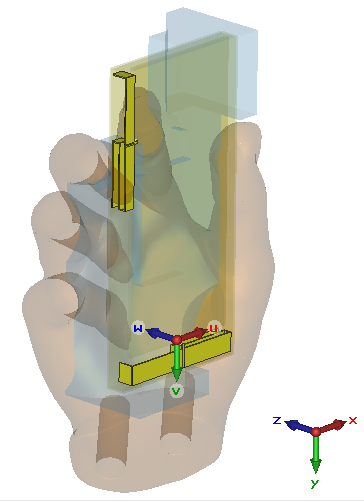
\includegraphics[width=\linewidth,height=4cm,keepaspectratio]{img/tech_sol/monopole/read_mode/3d_read_mode.PNG}
        \caption{Read mode.}
    \end{subfigure}
    \begin{subfigure}[b]{0.24\linewidth}
        \centering 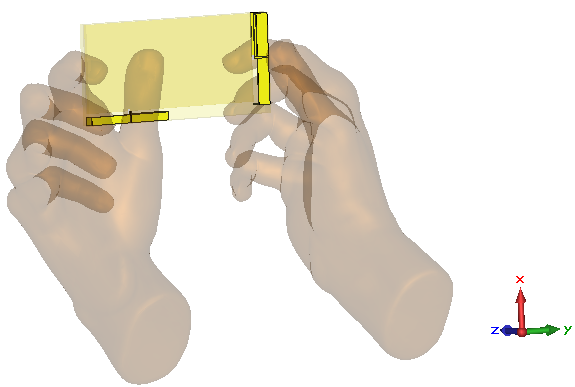
\includegraphics[width=\linewidth,height=4cm,keepaspectratio]{img/tech_sol/monopole/play_mode/3d_play_mode.PNG}
        \caption{Play mode.}
    \end{subfigure}
    \begin{subfigure}[b]{0.24\linewidth}
        \centering 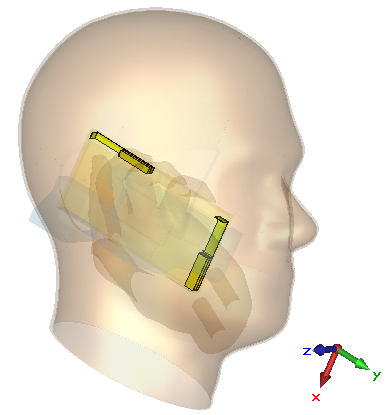
\includegraphics[width=\linewidth,height=4cm,keepaspectratio]{img/tech_sol/monopole/talk_mode/3d_talk_mode.PNG}
        \caption{Talk mode.}
    \end{subfigure}
    \begin{subfigure}[b]{0.24\linewidth}
        \centering 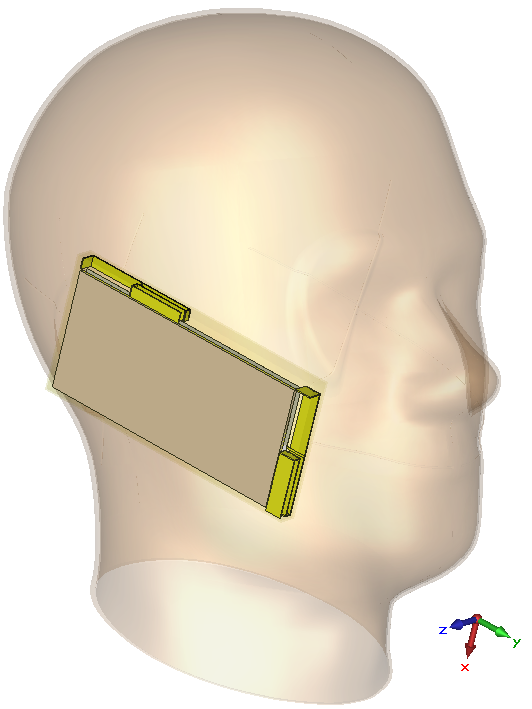
\includegraphics[width=\linewidth,height=4cm,keepaspectratio]{img/tech_sol/monopole/sar/3d_sar.PNG}
        \caption{SAR.}
    \end{subfigure}
    \caption{MIMO monopole antenna position for each user effect simulation.}
    \label{fig:sol1_monoant_positions}
\end{figure}

\subsection{Read Mode}
%S-parameter
The S-parameter sweeps for the read mode, can be seen on Figure \ref{fig:sparam_mono_read_mode}. The highest obtainable bandwidth for both antennas is found from the S-parameter sweep and is listed in Table \ref{tab:bw_sol1read}. The top antenna covers the required bandwidth in both the low and high band. However as seen in the Table \ref{tab:bw_sol1read} the side antenna only covers the bandwidth in the high band and the low band needs additional tuning to fulfill the bandwidth requirements. The S-parameter sweeps \ref{fig:sparam_mono_read_mode} also shows the $S_{21}$ isolation loss. The highest notable isolation loss is within the low band, at \SI{10}{dB} and \SI{8}{dB} for the top and side antenna respectively.       

The correlation between the top and side antenna can be seen in Figure \ref{fig:corr_sols_read}. The correlation is plotted sweeping the tunable capacitors of each antenna, while the other antenna is fixed with a tunable at \SI{0.3}{pF}. The correlation for the top and side antenna is below 0.5 for both the low and high band as desired.

\begin{table}[htbp]
  \centering
  \begin{tabular}{|l|l|r|r|r|}
    \hline
    Antenna & Band & Start [MHz] & Stop [MHz] & Bandwidth [MHz] \\
    \hline
    Top     & Low  &  677  & 1065  & 388 \\
    Side    & Low  &  700  & 710  & 10  \\
    \hline
    Top     & High &  1183 &  2127  & 944 \\
    Side    & High & 1765 &  2120 & 355 \\
    \hline
  \end{tabular}
  \caption{Monopole antenna in read mode. Maximum bandwidth obtained in the low and high band for the top and the side antenna, respectively.}    
\label{tab:bw_sol1read}
\end{table}

\begin{figure}[htbp]
   \begin{subfigure}[b]{0.49\linewidth}
        \centering
        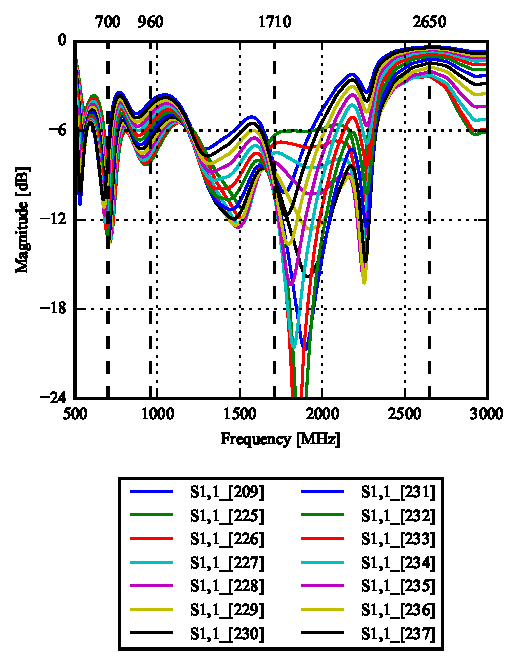
\includegraphics{img/tech_sol/monopole/read_mode/s11}
        \caption{$S_{11}$, sweeping $C_1$ and fixing $C_2$.}
    \end{subfigure}
    \hfill
    \begin{subfigure}[b]{0.49\linewidth}
        \centering
        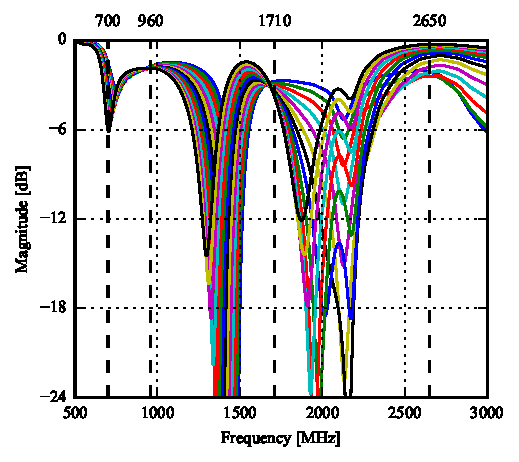
\includegraphics{img/tech_sol/monopole/read_mode/s22}
        \caption{$S_{22}$, sweeping $C_2$ and fixing $C_1$.}
    \end{subfigure}
~
    \begin{subfigure}[b]{0.49\linewidth}
        \centering
        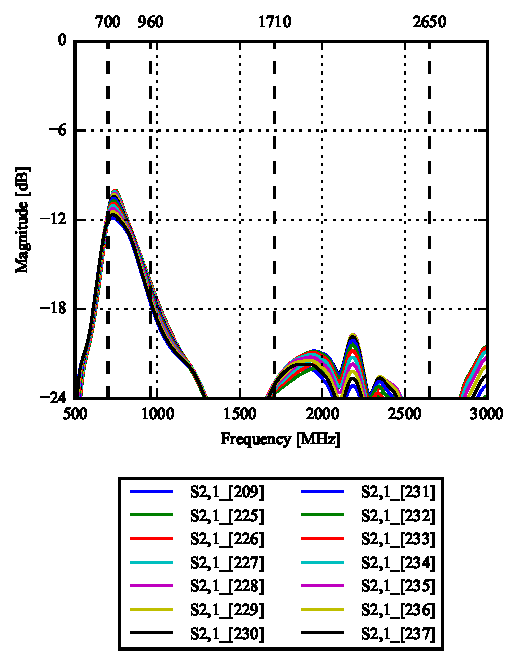
\includegraphics{img/tech_sol/monopole/read_mode/s21_s11}
        \caption{$S_{21}$, sweeping $C_1$ and fixing $C_2$.}
    \end{subfigure}
    \hfill
    \begin{subfigure}[b]{0.49\linewidth}
        \centering
        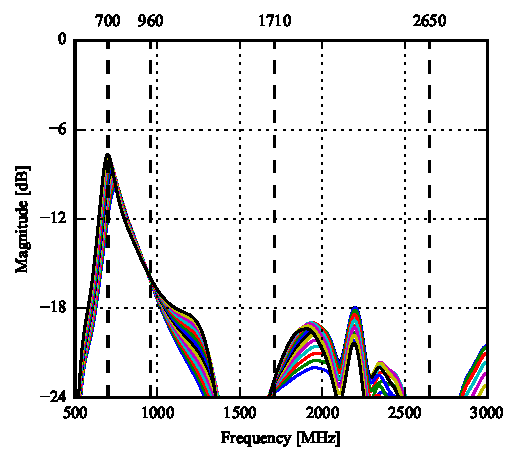
\includegraphics{img/tech_sol/monopole/read_mode/s21_s22}
        \caption{$S_{21}$, sweeping $C_2$ and fixing $C_1$.}
    \end{subfigure}
    \caption{Parameter sweep in read mode for tuning the shunt capacitor of each antenna, $C_1$ and $C_2$ for port 1 and 2, respectively. Port 1 is the top antenna and port 2 is the side antenna.}
    \label{fig:sparam_mono_read_mode}
\end{figure}

% Correlation
\begin{figure}[htbp]
    \centering
    \begin{subfigure}{0.49\linewidth}
        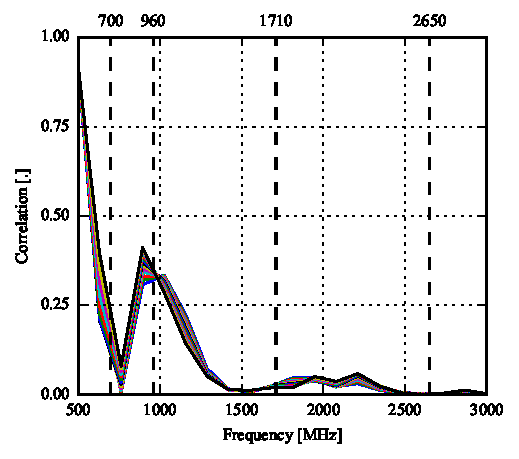
\includegraphics{img/tech_sol/monopole/read_mode/s11_corr}
        \caption{Sweeping $C_1$ and fixing $C_2$.}
    \end{subfigure}
    \hfill
    \begin{subfigure}{0.49\linewidth}
        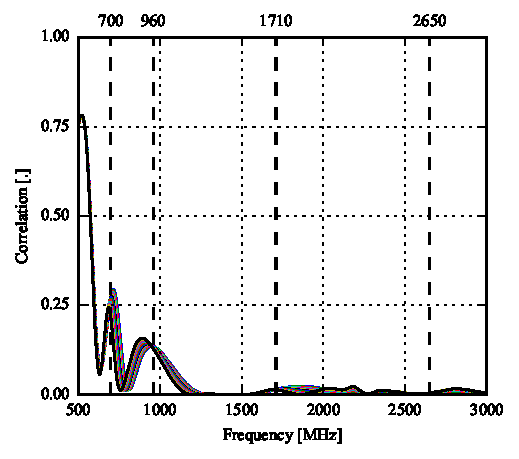
\includegraphics{img/tech_sol/monopole/read_mode/s22_corr}
        \caption{Sweeping $C_2$ and fixing $C_1$.}
    \end{subfigure}
    \caption{Monopole antenna in read mode. Correlation between antennas then sweeping tuning capacitors. Here, $C_1$ and $C_2$ are the tuning capacitor for the top and side antenna, respectively.}
    \label{fig:corr_sols_read}
\end{figure}

\subsection{Play Mode}
%S-parameter
The S-parameter sweeps for the read mode, can be seen on Figure \ref{fig:sparam_mono_play_mode}. The highest obtainable bandwidth for both antennas is found from the S-parameter sweep and is listed in Table \ref{tab:bw_sol1play}. The top antenna covers the required bandwidth in the low band but lacks \SI{87}{MHz} in the high band. The side antenna does not fulfill any of the bandwidth requirements and will need additional tuning. The S-parameter sweeps \ref{fig:sparam_mono_play_mode} also shows the $S_{21}$ isolation loss. The highest notable isolation loss is within the low band, at \SI{12}{dB} and \SI{10}{dB} for the top and side antenna respectively.       

The correlation between the top and side antenna can be seen in Figure \ref{fig:corr_sols_play}. The correlation is plotted sweeping the tunable capacitors of each antenna, while the other antenna is fixed with a tunable at \SI{0.3}{pF}. The correlation for the top and side exceeds the required correlation limit with 0.1 in the low band from \SI{700}{MHz} to \SI{880}{MHz}.
\begin{table}[htbp]
    \centering
    \begin{tabular}{|l|l|r|r|r|}
      \hline
      Antenna & Band & Start [MHz] & Stop [MHz] & Bandwidth [MHz] \\
      \hline
      Top     & Low  & 920 & 1000 &  80 \\
      Side    & Low  & 1010 & 1060 & 50 \\
      \hline
      Top     & High & 1420 & 2053 & 633 \\
      Side    & High & 1635 & 2180 & 545 \\
      \hline
    \end{tabular}
    \caption{Monopole antenna in play mode. Maximum bandwidth obtained in the low and high band for the top and the side antenna, respectively.}    \label{tab:bw_sol1play}
  \end{table}

  \begin{figure}[htbp]
    \begin{subfigure}[b]{0.49\linewidth}
      \centering
      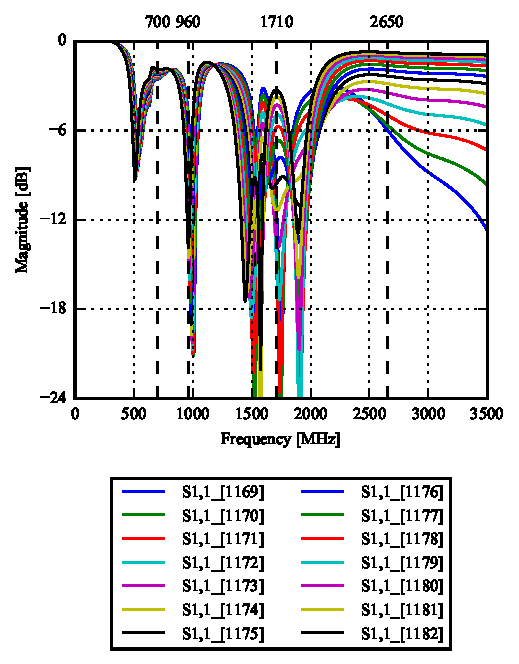
\includegraphics{img/tech_sol/monopole/play_mode/s11}
      \caption{$S_{11}$, sweeping $C_1$ and fixing $C_2$.}
    \end{subfigure}
    \hfill
    \begin{subfigure}[b]{0.49\linewidth}
        \centering
        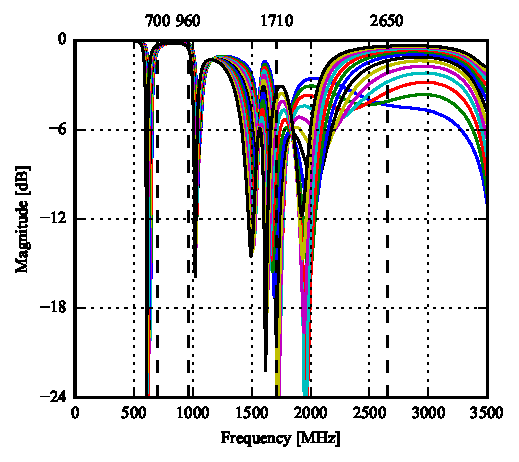
\includegraphics{img/tech_sol/monopole/play_mode/s22}
        \caption{$S_{22}$, sweeping $C_2$ and fixing $C_1$.}
    \end{subfigure}
~
    \begin{subfigure}[b]{0.49\linewidth}
        \centering
        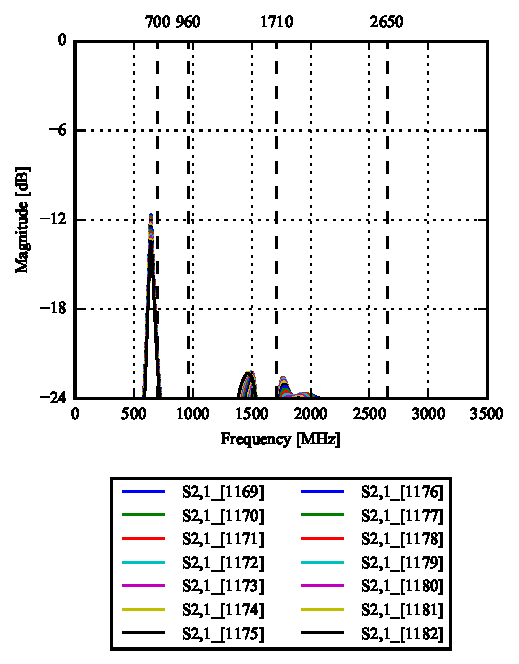
\includegraphics{img/tech_sol/monopole/play_mode/s21_s11}
        \caption{$S_{21}$, sweeping $C_1$ and fixing $C_2$.}
    \end{subfigure}
    \hfill
    \begin{subfigure}[b]{0.49\linewidth}
        \centering
        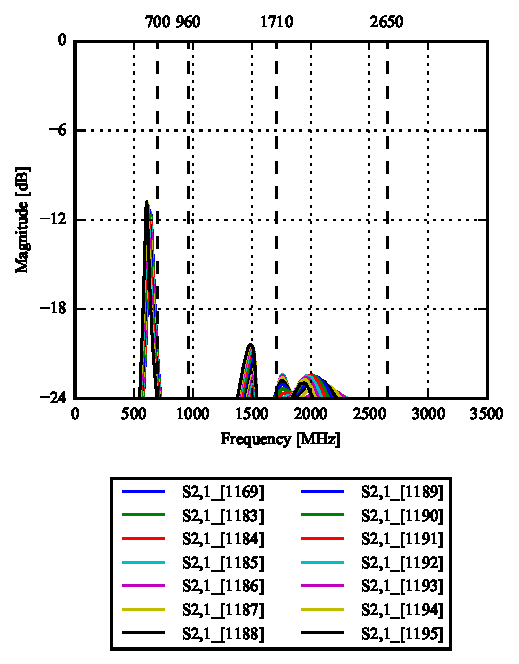
\includegraphics{img/tech_sol/monopole/play_mode/s21_s22}
        \caption{$S_{21}$, sweeping $C_2$ and fixing $C_1$.}
    \end{subfigure}
    \caption{Parameter sweep in play mode for tuning the shunt capacitor of each antenna, $C_1$ and $C_2$ for port 1 and 2, respectively. Port 1 is the top antenna and port 2 is the side antenna.}
    \label{fig:sparam_mono_play_mode}
\end{figure}

% Correlation
\begin{figure}[htbp]
    \centering
    \begin{subfigure}{0.49\linewidth}
        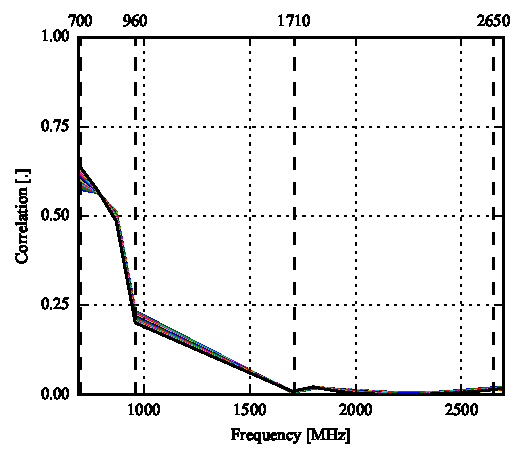
\includegraphics{img/tech_sol/monopole/play_mode/s11_corr}
        \caption{Sweeping $C_1$ and fixing $C_2$.}
    \end{subfigure}
    \hfill
    \begin{subfigure}{0.49\linewidth}
        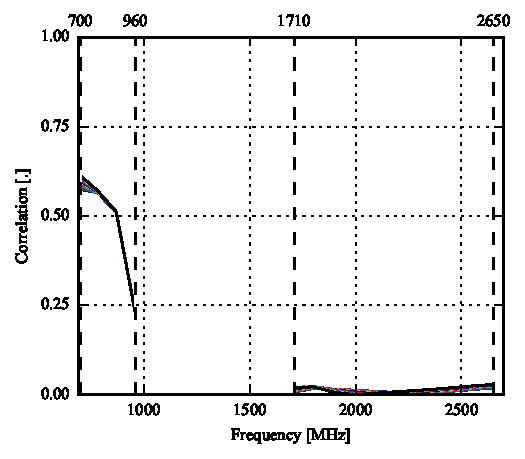
\includegraphics{img/tech_sol/monopole/play_mode/s22_corr}
        \caption{Sweeping $C_2$ and fixing $C_1$.}
    \end{subfigure}
    \caption{Monopole antenna in play mode. Correlation between antennas then sweeping tuning capacitors. Here, $C_1$ and $C_2$ are the tuning capacitor for the top and side antenna, respectively.}
    \label{fig:corr_sol1_play}
\end{figure}

\subsection{Talk Mode}
%S-parameter
The S-parameter sweeps for the read mode, can be seen on Figure \ref{fig:sparam_mono_talk_mode}. The highest obtainable bandwidth for both antennas is found from the S-parameter sweep and is listed in Table \ref{tab:bw_sol1talk}. The top antenna covers the required bandwidth in the low band but lacks \SI{87}{MHz} in the high band. The side antenna does not fulfill any of the bandwidth requirements and will need additional tuning. The S-parameter sweeps \ref{fig:sparam_mono_talk_mode} also shows the $S_{21}$ isolation loss. The highest notable isolation loss is within the low band, at \SI{13}{dB} and \SI{10}{dB} both the top and side antenna respectively.

The correlation between the top and side antenna can be seen in Figure \ref{fig:corr_sols_talk}. The correlation is plotted sweeping the tunable capacitors of each antenna, while the other antenna is fixed with a tunable at \SI{0.3}{pF}. The correlation for the top and side exceeds the required correlation limit with 0.1 in the low band from \SI{700}{MHz} to \SI{880}{MHz}.

%bandwidth
\begin{table}[htbp]
    \centering
    \begin{tabular}{|l|l|r|r|r|}
        \hline
        Antenna & Band & Start [MHz] & Stop [MHz] & Bandwidth [MHz] \\
        \hline
        Top     & Low  & 510 & 645  & 135 \\
        Side    & Low  & & & 0    \\
        \hline
        Top     & High & 1092 & 2305  & 1213 \\
        Side    & High & 1335  & 2132 & 797 \\
        \hline
    \end{tabular}
    \caption{Monopole antenna in talk mode. Maximum bandwidth obtained in the low and high band for the top and the side antenna, respectively.}    \label{tab:bw_sol1talk}
\end{table}

\begin{figure}[htbp]
   \begin{subfigure}[b]{0.49\linewidth}
        \centering
        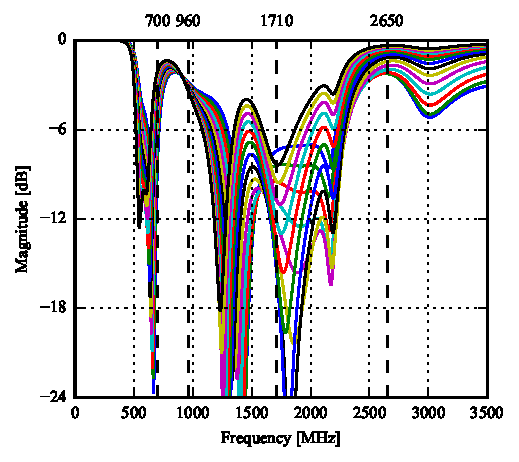
\includegraphics{img/tech_sol/monopole/talk_mode/s11}
        \caption{$S_{11}$, sweeping $C_1$ and fixing $C_2$.}
    \end{subfigure}
    \hfill
    \begin{subfigure}[b]{0.49\linewidth}
        \centering
        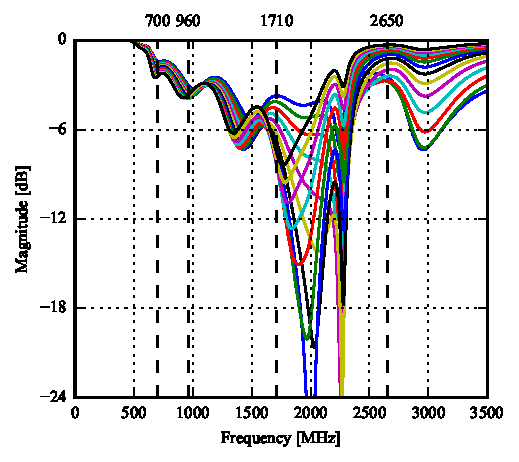
\includegraphics{img/tech_sol/monopole/talk_mode/s22}
        \caption{$S_{22}$, sweeping $C_2$ and fixing $C_1$.}
    \end{subfigure}
~
    \begin{subfigure}[b]{0.49\linewidth}
        \centering
        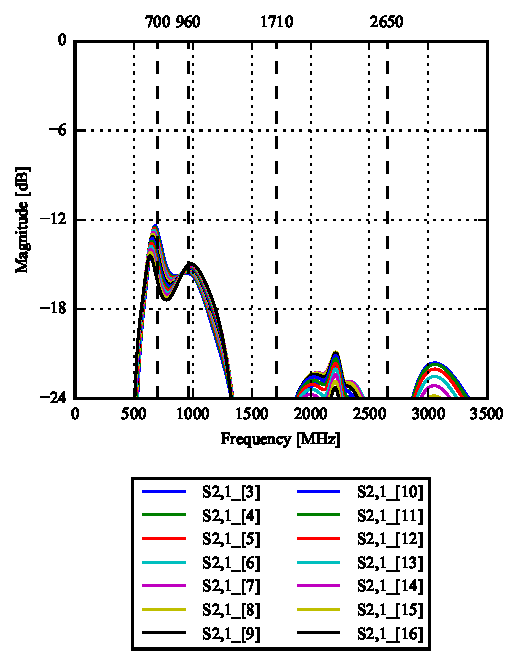
\includegraphics{img/tech_sol/monopole/talk_mode/s21_s11}
        \caption{$S_{21}$, sweeping $C_1$ and fixing $C_2$.}
    \end{subfigure}
    \hfill
    \begin{subfigure}[b]{0.49\linewidth}
        \centering
        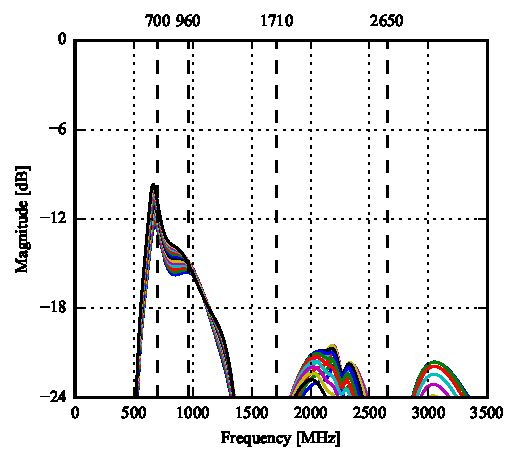
\includegraphics{img/tech_sol/monopole/talk_mode/s21_s22}
        \caption{$S_{21}$, sweeping $C_1$ and fixing $C_2$.}
    \end{subfigure}
    \caption{Parameter sweep for tuning the shunt capacitor of each antenna, $C_1$ and $C_2$ for port 1 and 2, respectively. Port 1 is the top antenna and port 2 is the side antenna.}
    \label{fig:sparam_mono_talk_mode}
\end{figure}
% Correlation
\begin{figure}[htbp]
    \centering
    \begin{subfigure}{0.49\linewidth}
        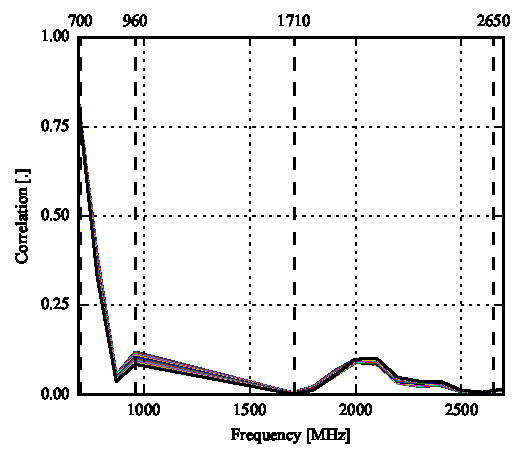
\includegraphics{img/tech_sol/monopole/talk_mode/s11_corr}
        \caption{Sweeping $C_1$ and fixing $C_2$.}
    \end{subfigure}
    \hfill
    \begin{subfigure}{0.49\linewidth}
        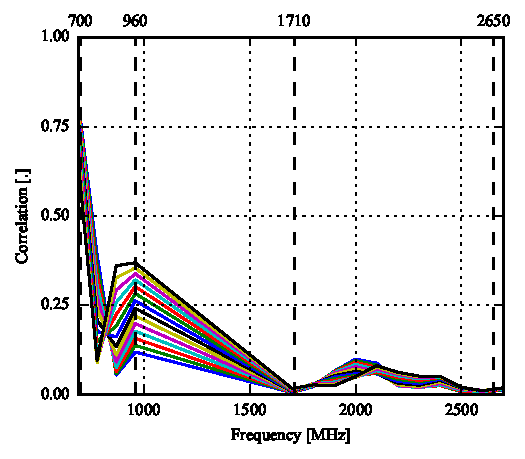
\includegraphics{img/tech_sol/monopole/talk_mode/s22_corr}
        \caption{Sweeping $C_2$ and fixing $C_1$.}
    \end{subfigure}
    \caption{Monopole antenna in read mode. Correlation between antennas then sweeping tuning capacitors. Here, $C_1$ and $C_2$ are the tuning capacitor for the top and side antenna, respectively.}
    \label{fig:corr_sol1_read}
\end{figure}

\subsection{SAR}

